% CVPR 2022 Paper Template
% based on the CVPR template provided by Ming-Ming Cheng (https://github.com/MCG-NKU/CVPR_Template)
% modified and extended by Stefan Roth (stefan.roth@NOSPAMtu-darmstadt.de)

\documentclass[10pt,twocolumn,letterpaper]{article}

%%%%%%%%% PAPER TYPE  - PLEASE UPDATE FOR FINAL VERSION
% \usepackage[review]{cvpr}      % To produce the REVIEW version
% \usepackage{cvpr}              % To produce the CAMERA-READY version
\usepackage[pagenumbers]{cvpr} % To force page numbers, e.g. for an arXiv version

% Include other packages here, before hyperref.
\usepackage{graphicx}
\usepackage{amsmath}
\usepackage{amssymb}
\usepackage{booktabs}

% It is strongly recommended to use hyperref, especially for the review version.
% hyperref with option pagebackref eases the reviewers' job.
% Please disable hyperref *only* if you encounter grave issues, e.g. with the
% file validation for the camera-ready version.
%
% If you comment hyperref and then uncomment it, you should delete
% ReviewTempalte.aux before re-running LaTeX.
% (Or just hit 'q' on the first LaTeX run, let it finish, and you
%  should be clear).
\usepackage[pagebackref,breaklinks,colorlinks]{hyperref}


% Support for easy cross-referencing
\usepackage[capitalize]{cleveref}
\crefname{section}{Sec.}{Secs.}
\Crefname{section}{Section}{Sections}
\Crefname{table}{Table}{Tables}
\crefname{table}{Tab.}{Tabs.}


%%%%%%%%% PAPER ID  - PLEASE UPDATE
\def\cvprPaperID{0}
\def\confName{CSE 559a}
\def\confYear{2023}


\begin{document}

%%%%%%%%% TITLE - PLEASE UPDATE
\title{Project Proposal: One-stage method for open-vocabulary semantic segmentation by soliciting co-existing object relations}

\author{
Tovi Tu \hspace{1in} Anthony Chen \hspace{1in} Shuhan(Steven) Zhang  \hspace{1in} Ben Mueller 
}
\maketitle

%%%%%%%%% ABSTRACT
\begin{abstract}
  Your abstract goes here.
\end{abstract}

%%%%%%%%% BODY TEXT
\section{Project Overview}

\subsection{Motivation}

Semantic segmentation is a fundamental computer vision task being studied extensively in a fixed-category setting. However, past models with prediction heads trained in an end-to-end manner lack the flexibility to be readily applied to real-world scenarios. Recent advancements in image encoders supervised by natural language captions have demonstrated amazing abilities to learn cross-modal embeddings adaptable to various downstream tasks. The embedded semantics for a wide range of common objects can effectively extend the image classes beyond predetermined categories. 

\subsection{Problem Definition}

Open-vocabulary semantic segmentation falls into the category of zero-shot learning. This task challenges a model to assign pixel-level class labels from $C=C_{seen} \cup C_{unseen}$ to a given image $x\in X$, where $C_{seen}$ and $C_{unseen}$ are mutually exclusive sets and the former represents classes available in the training set $X_{train}$. The model is trained on $X_{train}$, with input images and ground truth annotation masks. During test time, the model is evaluated in a zero-shot setting, trying to correctly predict unseen labels $c\in C_{unseen}$ in addition to seen labels in the training set $X_{test}$. 

\subsection{Related Works}

A previous method, SimSeg \cite{simseg}, has successfully adapted pretrained CLIP models \cite{clip} for open-vocabulary segmentation by first predicting a class-agnostic mask and then classifying each masked image with CLIP. Since the vanilla CLIP model is trained to generate a global feature for any image, there is a granularity gap between the pretraining objective and the more fine-grained semantic segmentation objective. To close the gap, SimSeg complements MaskFormer \cite{maskformer}, a fixed-class segmentation model, with CLIP to extend the possible classes. However, it fails to exploit the relational information of objects present in the scene by categorizing one masked image at step.

\subsection{Proposed Method}

Inspired by the distributional semantics theory, we propose to capture the distribution of co-existing objects in a scene. In a natural setting, objects in an image often appear together and collectively determine the overall context. Figure 1 gives an intuitive example. In a scenic shot, the appearance of a sea increases the probability of seeing a beach, and a hill is likely to be accompanied by clouds or the sky. The collection of the co-existing objects defines an abstract context of outdoor scenery and rules out the probability of seeing indoor concepts such as a sofa or a television. 

Building upon the intuition, we propose a one-stage architecture that segments an object from the image auto-progressively by first targeting the most prominent object and then conditioning subsequent predictions on previous results. As a preliminary thought, we envision this model to have a transformer style and use a pretrained CLIP encoder and ClipSeg \cite{clipseg} decoder, a zero-shot semantic segmentation model conditioned on prompts, as the backbone. We will modify the encoder for the support prompt to predict the most probable object at the current timestep, which is different from those predicted in the previous timesteps. For the first prediction, we would condition the prediction on a learnable token to signify the start of the sequence and update it during training. We consider freezing those modules or finetuning them with a lower learning rate to avoid catastrophic forgetting in the backbone model.

\begin{figure} [h]
    \centering
    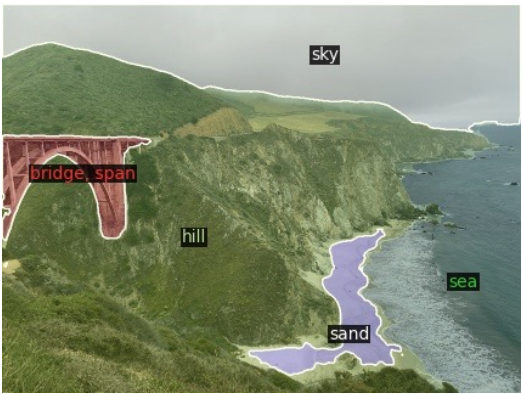
\includegraphics[width=0.5\linewidth]{images/seg_sample.png}
    \caption{Enter Caption}
    \label{fig:enter-label}
\end{figure}
 

\section{Team Member Roles/Tasks}
\label{sec:roles}
Following the structure for machine learning tasks, we have separated our overall project into 4 sections, data, architecture, training, and benchmark. However, since data and benchmark are tightly coupled, we will combine them into one cohesive section. The detailed responsibility + assignment is outlined below:

\subsection{Tovi Tu - Architecture}

 The architecture lead is responsible for designing the overall structure of the models, including selecting the framework, algorithms, and methodologies. This is crucial and technically complex, which is why we assigned the task to our most technically familiar member in this field, Tovy.


\subsection{Anthony Chen - Training}
The training lead is responsible for developing and implementing the training procedure, optimizing model, and ensuring that the training is effective using the datasets. Since this involves more python familiarity and access to computational resources, this task is delegated to Anthony.


\subsection{Steven Zhang - Data}

Data lead is responsible for researching, collecting, preprocessing, and augmenting datasets for the training procedures. This would require more research and data science expertise. 


\subsection{Ben Mueller - Benchmark}

As of bench-marking, where the lead is responsible for running related work’s code on the predefined datasets to acquire benchmarks comparison, as well as running our model on multiple datasets to ensure quality and effectiveness. 



\section{Resources}
\begin{itemize}
    \item Computational
    \begin{itemize}
        \item Graphics
        \item RIS + Research lab resources
        \item Google Colab Credits if needed
    \end{itemize}
    \item Data:
    \begin{itemize}
        \item Open Vocabulary Semantic Segmentation \\
        \url{https://paperswithcode.com/task/open-vocabulary-semantic-segmentation}
    \end{itemize}
    \item Outside code
    \begin{itemize}
        \item A Simple Baseline for Open Vocabulary Semantic Segmentation with Pre-trained Vision-language Model \\
        \url{https://github.com/mendelxu/zsseg.baseline}
    \end{itemize}
\end{itemize}

\section{Reservations}

One major reservation that we have with this project is that we won’t be able to fully anticipate the computational (training) complexity until we perform further experimentation. As such, the datasets we plan to use may be too large for us to complete comprehensive training and benchmarking using the compute resources at our disposal. If this becomes a problem, we hope that for a minimal goal we will at least have a working re-implementation of the baseline model’s architecture (\url{https://github.com/MendelXu/zsseg.baseline?tab=readme-ov-file}) and to be able to benchmark it on at least one of the datasets that we have brought in. Similarly, a slight reservation we have is the time required to perform all of the needed benchmarking \& training for these models, which is another reason that we want to keep this minimal goal in mind. 
\begin{itemize}
    \item Won’t be able to fully anticipate computational+training complexity until further experimentation.
    \item The dataset might be overly large to complete comprehensive training/benchmarking.
    \item Minimal:
    \begin{itemize}
        \item Implementation of the simple baseline’s architecture. \url{https://github.com/MendelXu/zsseg.baseline?tab=readme-ov-file}
        \item Benchmark on at least one of the dataset.
    \end{itemize}
\end{itemize}


\section{Relationship to Background}

\begin{itemize}
    \item \textbf{Tovi} - Currently working on vision-language models under supervision of Prof. Chenguang Wang as an independent project; experience with machine learning and deep learning in time-series analysis and classification.
    \item \textbf{Anthony} - Taking NLP and CV, familiar with the ML training process. Currently working as a Tech Lead in an iOS application project from WashU medical school. Have more experiences on the tech side: code, GPU, data storing, interface.
    \item \textbf{Steven} - Steven is experienced with pytorch and related frameworks. Moreover, through past independent research experiences in both WUSTL and Peking University, Steven is familiar with research methodologies related with image search tasks and the utilization CLIP. Steven is not quite familiar with deep learning, or the latest methodologies in computer vision.
    \item \textbf{Ben} - Experience training large scale models using pytorch / pytorch lightning in research settings, currently using these in a Bioinformatics/ML research project in the WashU medical school.
\end{itemize}



%%%%%%%%% REFERENCES
{\small
\bibliographystyle{ieee_fullname}
\bibliography{bibliography}
}

\end{document}
